\chapter{Аналитический раздел}

В данном разделе будет проанализирована поставленная задача и рассмотрены различные способы ее реализации.

В ходе выполнения курсовой работы должно быть спроектировано и реализовано Web-приложение, позволяющее пользователю ознакомиться с прогнозами курса акций различных аналитиков. Пользователь должен иметь возможность получения прогнозируемой цены одной из предложенных акций. 
Кроме того, необходимо разработать ролевую модель, на основе которой будет строиться взаимодействие с веб-приложением. Предусмотреть три роли: пользователь, аналитик и администратор. Также необходимо создать систему регистрации и авторизации пользователей и предусмотреть возможность назначения ролей администратором. Сделать возможным для аналитика добавление, редактирование и удаление прогнозов.


\section{Формализация данных} 
В базе данных должна содержаться информация о:
\begin{itemize}
	\item компаниях;
 	\item прогнозах;
  \item финансовых показателях компаний;
  \item новостях компаний;
  \item пользователях;
  \item группах пользователей;
  \item правах доступа пользователей.  
\end{itemize}


\begin{table}[H]
	\centering
	\caption{Категории данных и сведения о них}
	\label{tbl:categories}
	\resizebox{\textwidth}{!}{%
		\begin{tabular}{|l|l|}
			\hline
			\textbf{\begin{tabular}[c]{@{}c@{}}Категория\end{tabular}} & \textbf{Сведения}  \\ \hline
			Компания & ID компании, название, логотип, описание, тикер, ID показателей \\ \hline
			Новость & ID новости, заголовок, дата публикации, наполнение, ссылка на источник, \\ & автор, ID компании  \\ \hline
			Прогноз & ID прогноза, инвест-дом, дата публикации, дата обновления, дата истечения, \\ & целевая цена, прогноз, описание прогноза, ID компании  \\ \hline
			Финансовые & ID показателей, цена, капитализация, объем прибыли до вычета налогов, \\ показатели & годовая выручка \\ \hline
			Пользователь & ID пользователя, имя пользователя в системе, пароль, \\  & электронная почта, полное имя \\ \hline
			Группа пользователей & ID записи, ID прав доступа, ID пользователя  \\ \hline
			Права доступа & ID записи, права доступа \\ \hline
		\end{tabular}%
	}
\end{table}


\section{Формализация ролей}
Должно быть выделено три категории пользователей.

\begin{table}[H]
	\centering
	\caption{Роли пользователей и предоставляемый им функционал}
	\label{tbl:roles_categories}
	\resizebox{\textwidth}{!}{%
		\begin{tabular}{|l|l|}
			\hline
			\textbf{\begin{tabular}[c]{@{}c@{}}Роль\end{tabular}} & \textbf{Функционал}  \\ \hline
			Пользователь & просмотр компаний и информации о них, просмотр предоставленных прав доступа \\ & просмотр прогнозов на выбранную компанию, просмотр новостей о компании \\ \hline
			Аналитик & добавление, просмотр, редактирование, удаление компаний, информации о них, \\ & а также прогнозов и новостей на выбранную компанию \\ \hline
			Администратор & просмотр, добавление, редактирование, удаление выбранных пользователей \\ & и прав доступа \\ \hline
		\end{tabular}%
	}
\end{table}

\newpage

\begin{figure}[h!]
	\begin{center}
		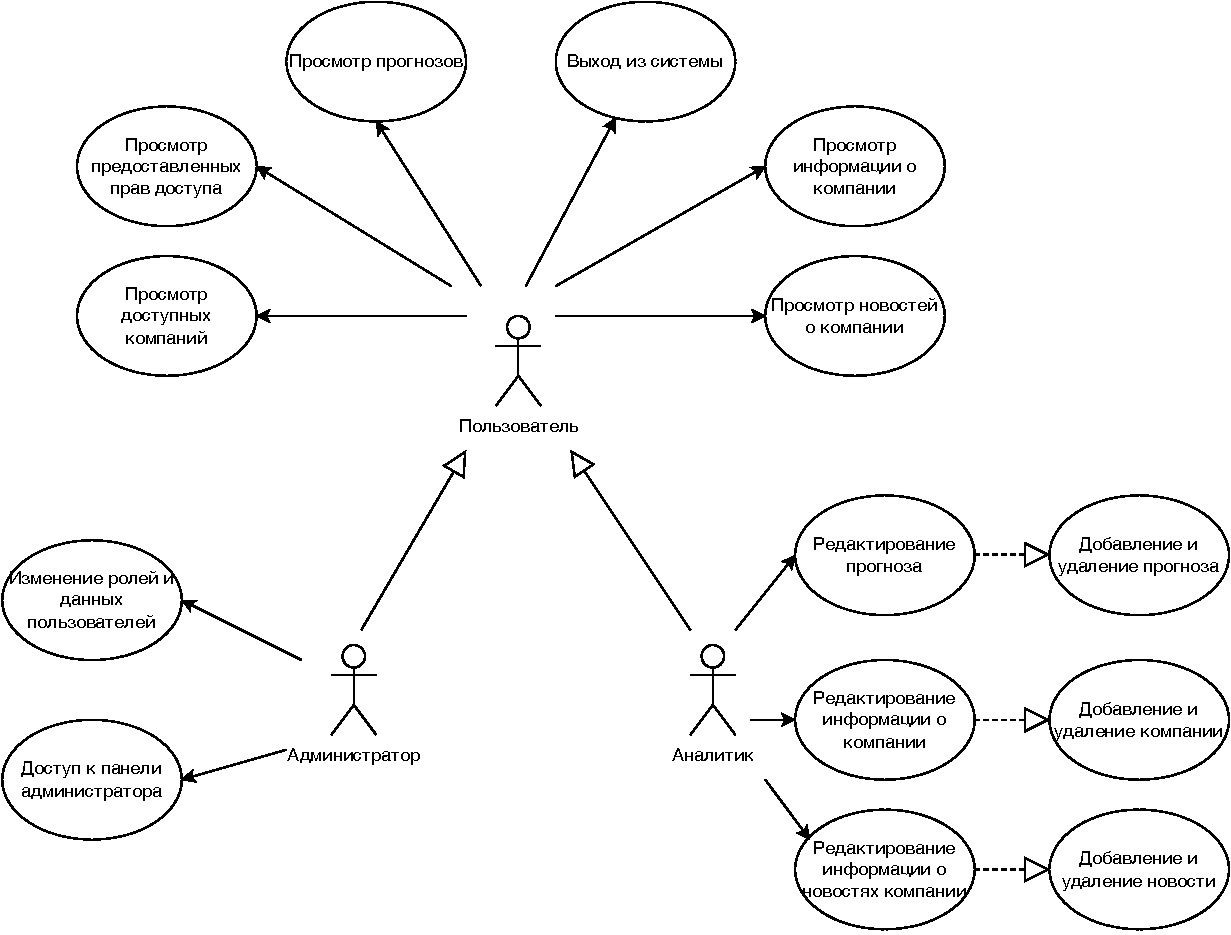
\includegraphics[scale=0.76]{inc/img/use-case.pdf}
	\end{center}
	\captionsetup{justification=centering}
	\caption{Диаграмма сценариев для пользователей, аналитиков и администратора}
	\label{img:use-case}
\end{figure}


\newpage
\section{Формализация сущностей системы}
На рисунках \ref*{img:er1} и \ref*{img:er2} отображены диаграммы сущностей системы. Данные диаграммы построены на основе данных таблицы \ref*{tbl:categories}.
\begin{figure}[h!]
	\begin{center}
		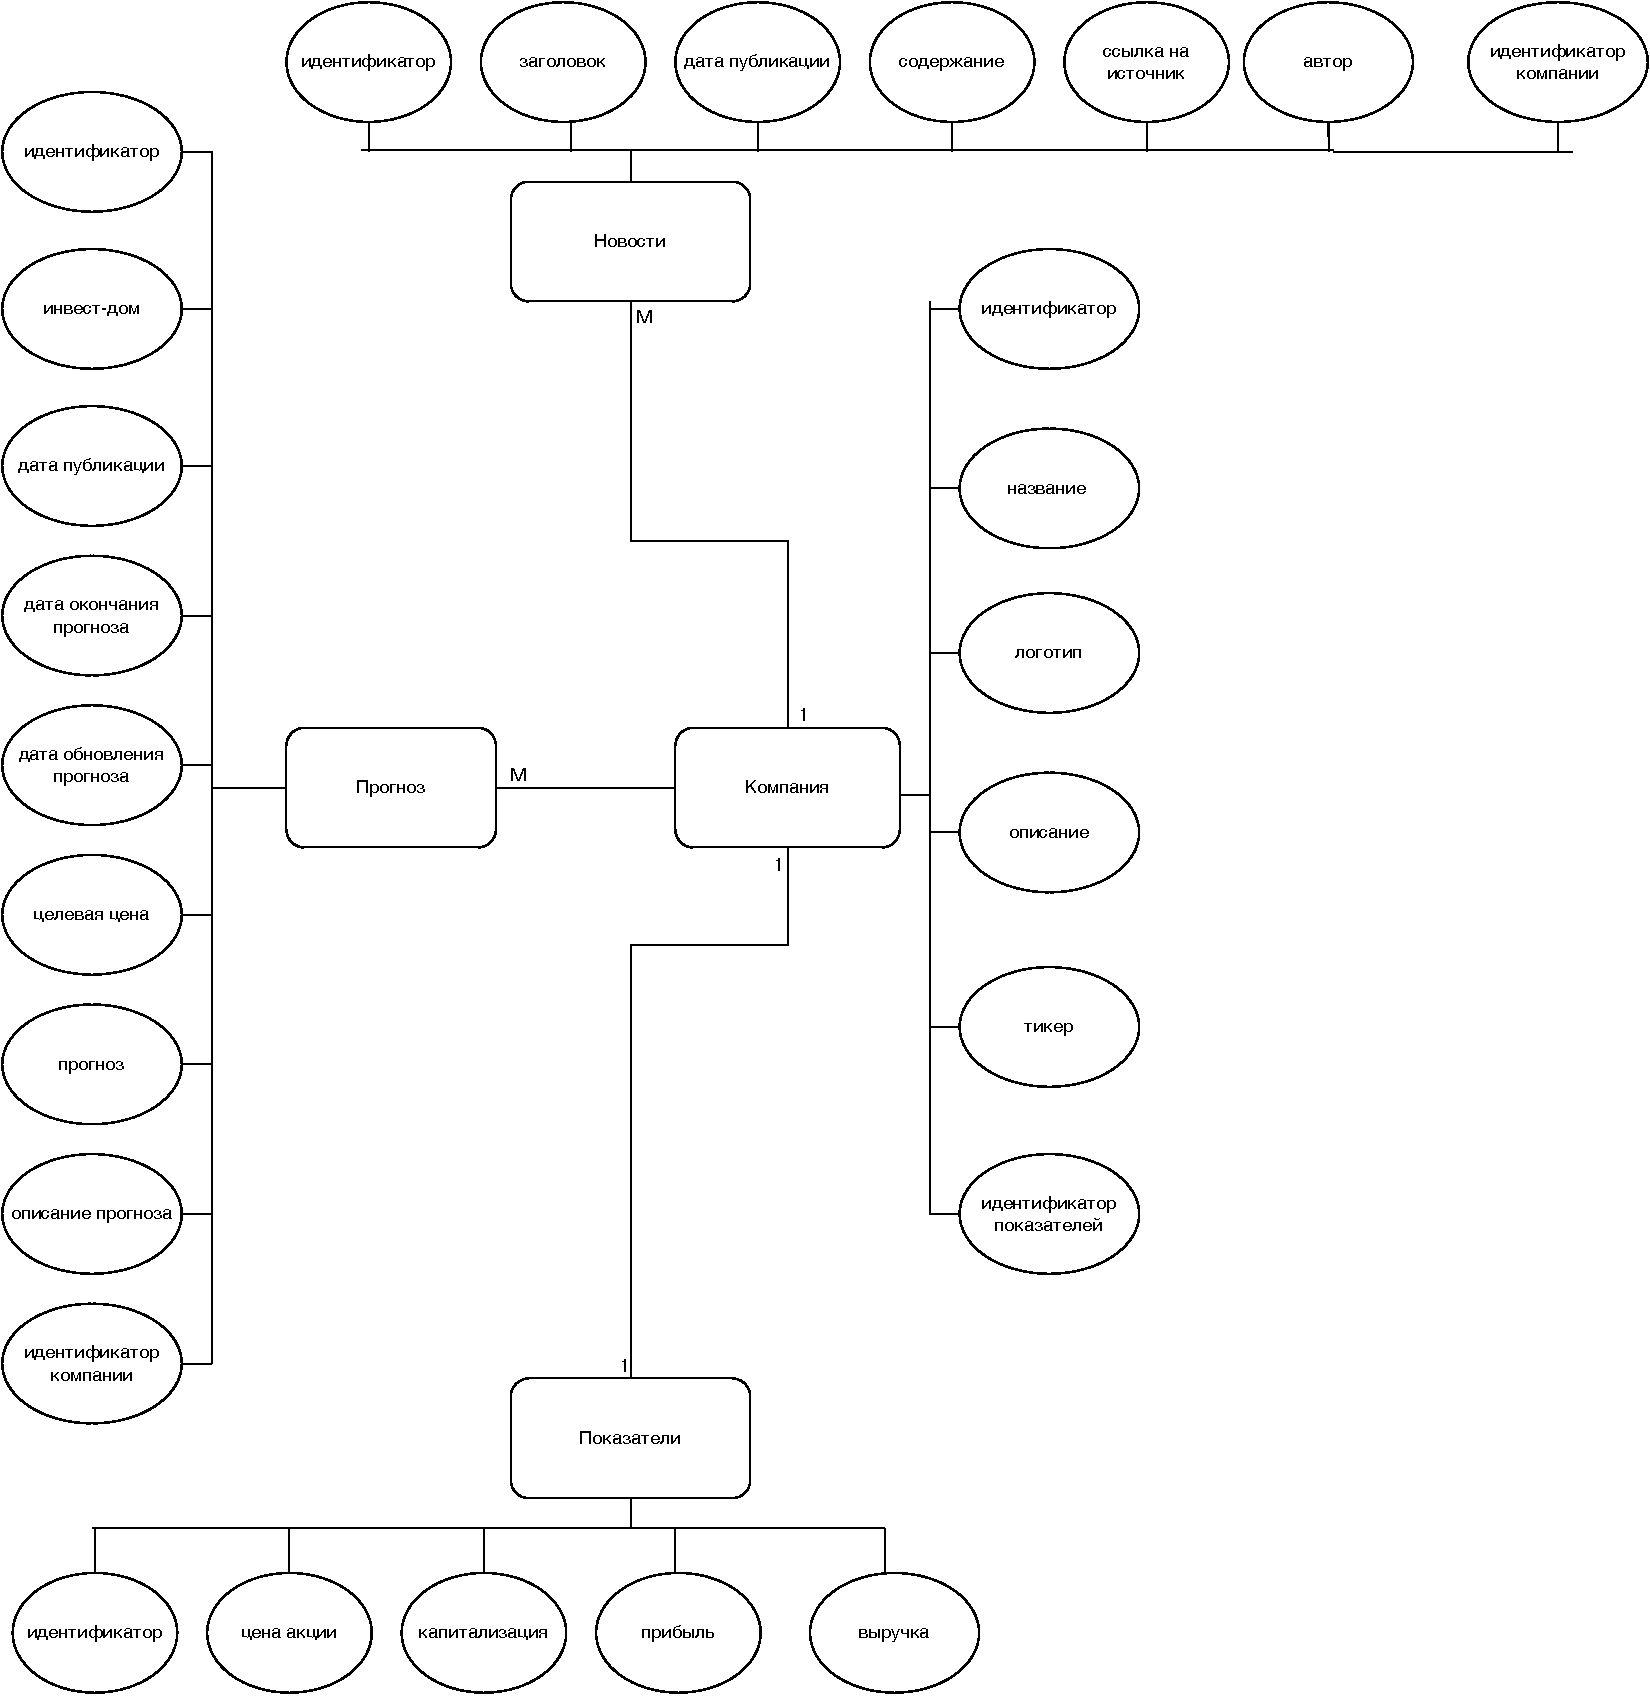
\includegraphics[scale=0.6]{inc/img/er.pdf}
	\end{center}
	\captionsetup{justification=centering}
	\caption{ER-диаграмма сущностей базы данных в нотации Чена (1)}
	\label{img:er1}
\end{figure}
\newpage


\begin{figure}[h!]
	\begin{center}
		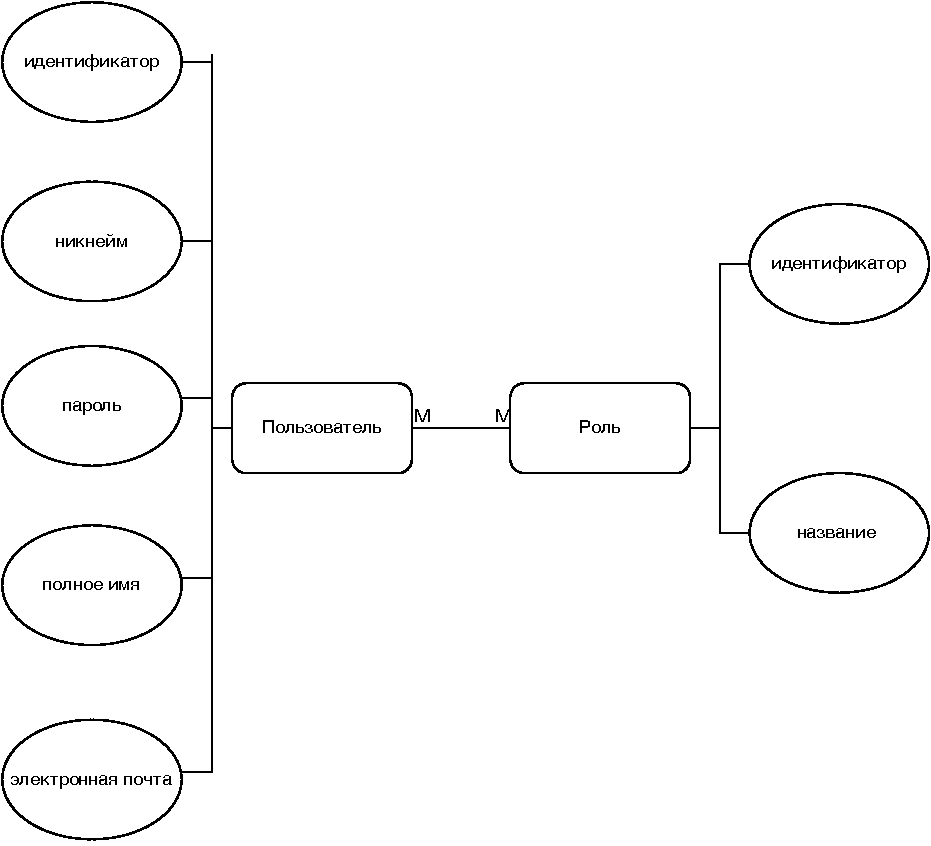
\includegraphics[scale=0.8]{inc/img/er2.pdf}
	\end{center}
	\captionsetup{justification=centering}
	\caption{ER-диаграмма сущностей базы данных в нотации Чена (2)}
	\label{img:er2}
\end{figure}



\section{Выбор модели хранения данных}

Модель данных --- это абстрактное, логическое определение объектов, операторов и прочих элементов, в совокупности состовляющих абстрактную машину доступа к данным, с которой взаимодействует пользователь. Эти объекты позволяют моделировать структуру данных, а операторы --- поведение данных \cite{1}.  

Существуют три основные модели данных:

\begin{itemize}
	\item иерархическая --- база данных с древовидной структурой с дугами --- связями и узлами --- элементами данных. Основной недостаток данной модели --- подобная структура не удовлетворяет требованиям многих задач \cite{2};
 	\item сетевая. В сетевой модели наряду с вертикальными связями допустимы и горизонтальные связи. Главный недостаток данной модели --- необходимость четко определять на физическом уровне связи данных и столь же четко следовать этой структуре свзяей при запросах к базе;
  	\item реляционная. Главное отличие состоит в том, что в данной модели информация хранится в виде таблиц, состоящих из нескольких записей --- кортежей, обладающих одним и тем же набором атрибутов или полей.  
\end{itemize}

Реляционная модель данных имеет ряд преимуществ в сравнении с остальными рассмотренными моделями, поскольку она более гибкая и удобная в использовании. Также она лучше всего соответствует описанным ранее связям между сущностями.



\section{Анализ существующих решений}
На сегодняшний день имеются различные сервисы, решающие поставленную цель в разной степени. Для их анализа введем следующие критерии: 
\begin{itemize}
	\item детализация --- приведение обширного количества информации о рассматриваемой компании;
 	\item аргументация --- автор прогноза обосновывает свой выбор;
  	\item объективность --- автор относится к рассматриваемой компании безэмоционально;
   	\item платный доступ --- просмотр прогнозов некторых компаний ограничен в бесплатной версии.
\end{itemize}
В качестве существующих решений для анализа выбраны сервисы Tinkoff Инвестиции, RBC Инвестиции, Investing.com, Finam.
В таблице \ref*{tbl:comparison} предствален сравнительный анализ существующих решений.

\begin{table}[H]
	\centering
	\caption{Анализ существующих решений}
	\label{tbl:comparison}
	\resizebox{\textwidth}{!}{%
		\begin{tabular}{|c|c|c|c|c|}
			\hline
			\textbf{Сервис} & \textbf{Деталиазация} & \textbf{Аргументация} & \textbf{Объективность} & \textbf{Платный доступ} \\ \hline
			Tinkoff Инвестиции                     & Да             & Нет            & Да                    & Нет           \\ \hline
			RBC Инвестиции                     & Нет             & Нет            & Нет                    & Нет           \\ \hline
			Investing.com                     & Да             & Нет             & Да                    & Да           \\ \hline
			Finam                			& Да             & Да             & Нет                   & Нет           \\ \hline
		\end{tabular}%
	}
\end{table}


\section*{Вывод}

В данном разделе была рассмотрена структура поставленной задачи, формализованны данные, используемые в системе, а также приведен анализ существующих решений.
